\documentclass{beamer}
\usetheme{Boadilla}
\setbeamertemplate{navigation symbols}{}

\usepackage[light]{antpolt}
\usepackage{amsmath}
\usepackage{tikz}

\newcommand{\eq}[1]{\begin{align*} #1 \end{align*}}
\newcommand{\game}[8]{\eq{\begin{array}{ccccccccc} \text{I} & #1 && #3 && #5 && #7\\ \text{II} && #2 && #4 && #6 && #8 \end{array}}}

\title[Playing games until the end of time]{Playing games until the end of time\\ {\small\textsc{Mingle '18}}}
\author[Dan Saattrup Nielsen]{Dan Saattrup Nielsen\\ University of Bristol}
\date{September 27, 2018}


\begin{document}

\begin{frame}
	\titlepage
\end{frame}

\begin{frame}{Let's play a stupid game}
	\begin{center}
		\pause I pick a natural number $n_0$\\\vspace{.2cm}
		\pause You pick another natural number $n_1$\\\vspace{.2cm}
		\pause You win if $n_1>n_0$
	\end{center}
\end{frame}

\begin{frame}{Let's model the \only<8->{\alert<8>{generalised} }stupid game}
	\game{\onslide<2->{n_0}}{\onslide<3->{n_1}}{\onslide<8->{\alert<8>{n_2}}}{\onslide<8->{\alert<8>{n_3}}}{\onslide<8->{\alert<8>{\cdots}}}{\onslide<8->{\alert<8>{\cdots}}}{\onslide<8->{\alert<8>{n_{2k}}}}{\onslide<8->{\alert<8>{n_{2k+1}}}}
	\onslide<4-7>{\hspace{2.9cm}$\underbrace{\phantom{aaaaaa}}_\text{1 round}$}
	\onslide<8>\hspace{-1.4cm}$\underbrace{\phantom{aaaaaaaaaaaaaaaaaaaaaaaaaaaaaaaaaaaa}}_\text{k+1 rounds}$\\\vspace{.2cm}

	\begin{center}
		\onslide<5-> You always have a \alert<5>{winning strategy}\\\vspace{.2cm}
		\onslide<6-> \only<1-5>{\phantom{For every $n_0$ there's an $n_1$ such that $n_1>n_0$}} \only<6>{For every $n_0$ there's an $n_1$ such that $n_1>n_0$}
		\only<7>{$\forall n_0\exists n_1: n_1>n_0$}
		\only<8>{$\forall n_0\exists n_1\alert<8>{\forall n_2\exists n_3\cdots\forall n_{2k}\exists n_{2k+1}}: n_{2k+1}>n_{2k}$}
	\end{center}
\end{frame}

\begin{frame}{Why are we playing\only<1>{ stupid}\only<2->{ silly} games?}
	\begin{center}
		\only<1>{\begin{center}\textit{First of all, games aren't stupid. Calm down.}\end{center}}
		\onslide<2-> We saw that player II has a winning strategy iff $\forall n_0\exists n_1\forall n_2\exists n_3\cdots\forall n_{2k}\exists n_{2k+1}: n_{2k+1}>n_{2k}$\\\vspace{.5cm}
		\onslide<3-> Analogously, player I has a winning strategy iff $\exists n_0\forall n_1\exists n_2\forall n_3\cdots\exists n_{2k}\forall n_{2k+1}: n_{2k+1}\leq n_{2k}$\\\vspace{.8cm}
		\onslide<4-> But these two are just negations of each other, so one of them is true\\\vspace{.1cm}
		\onslide<5-> We say that finite games are \alert{determined}
	\end{center}
\end{frame}

\begin{frame}{Chess is determined}
	\begin{center}
		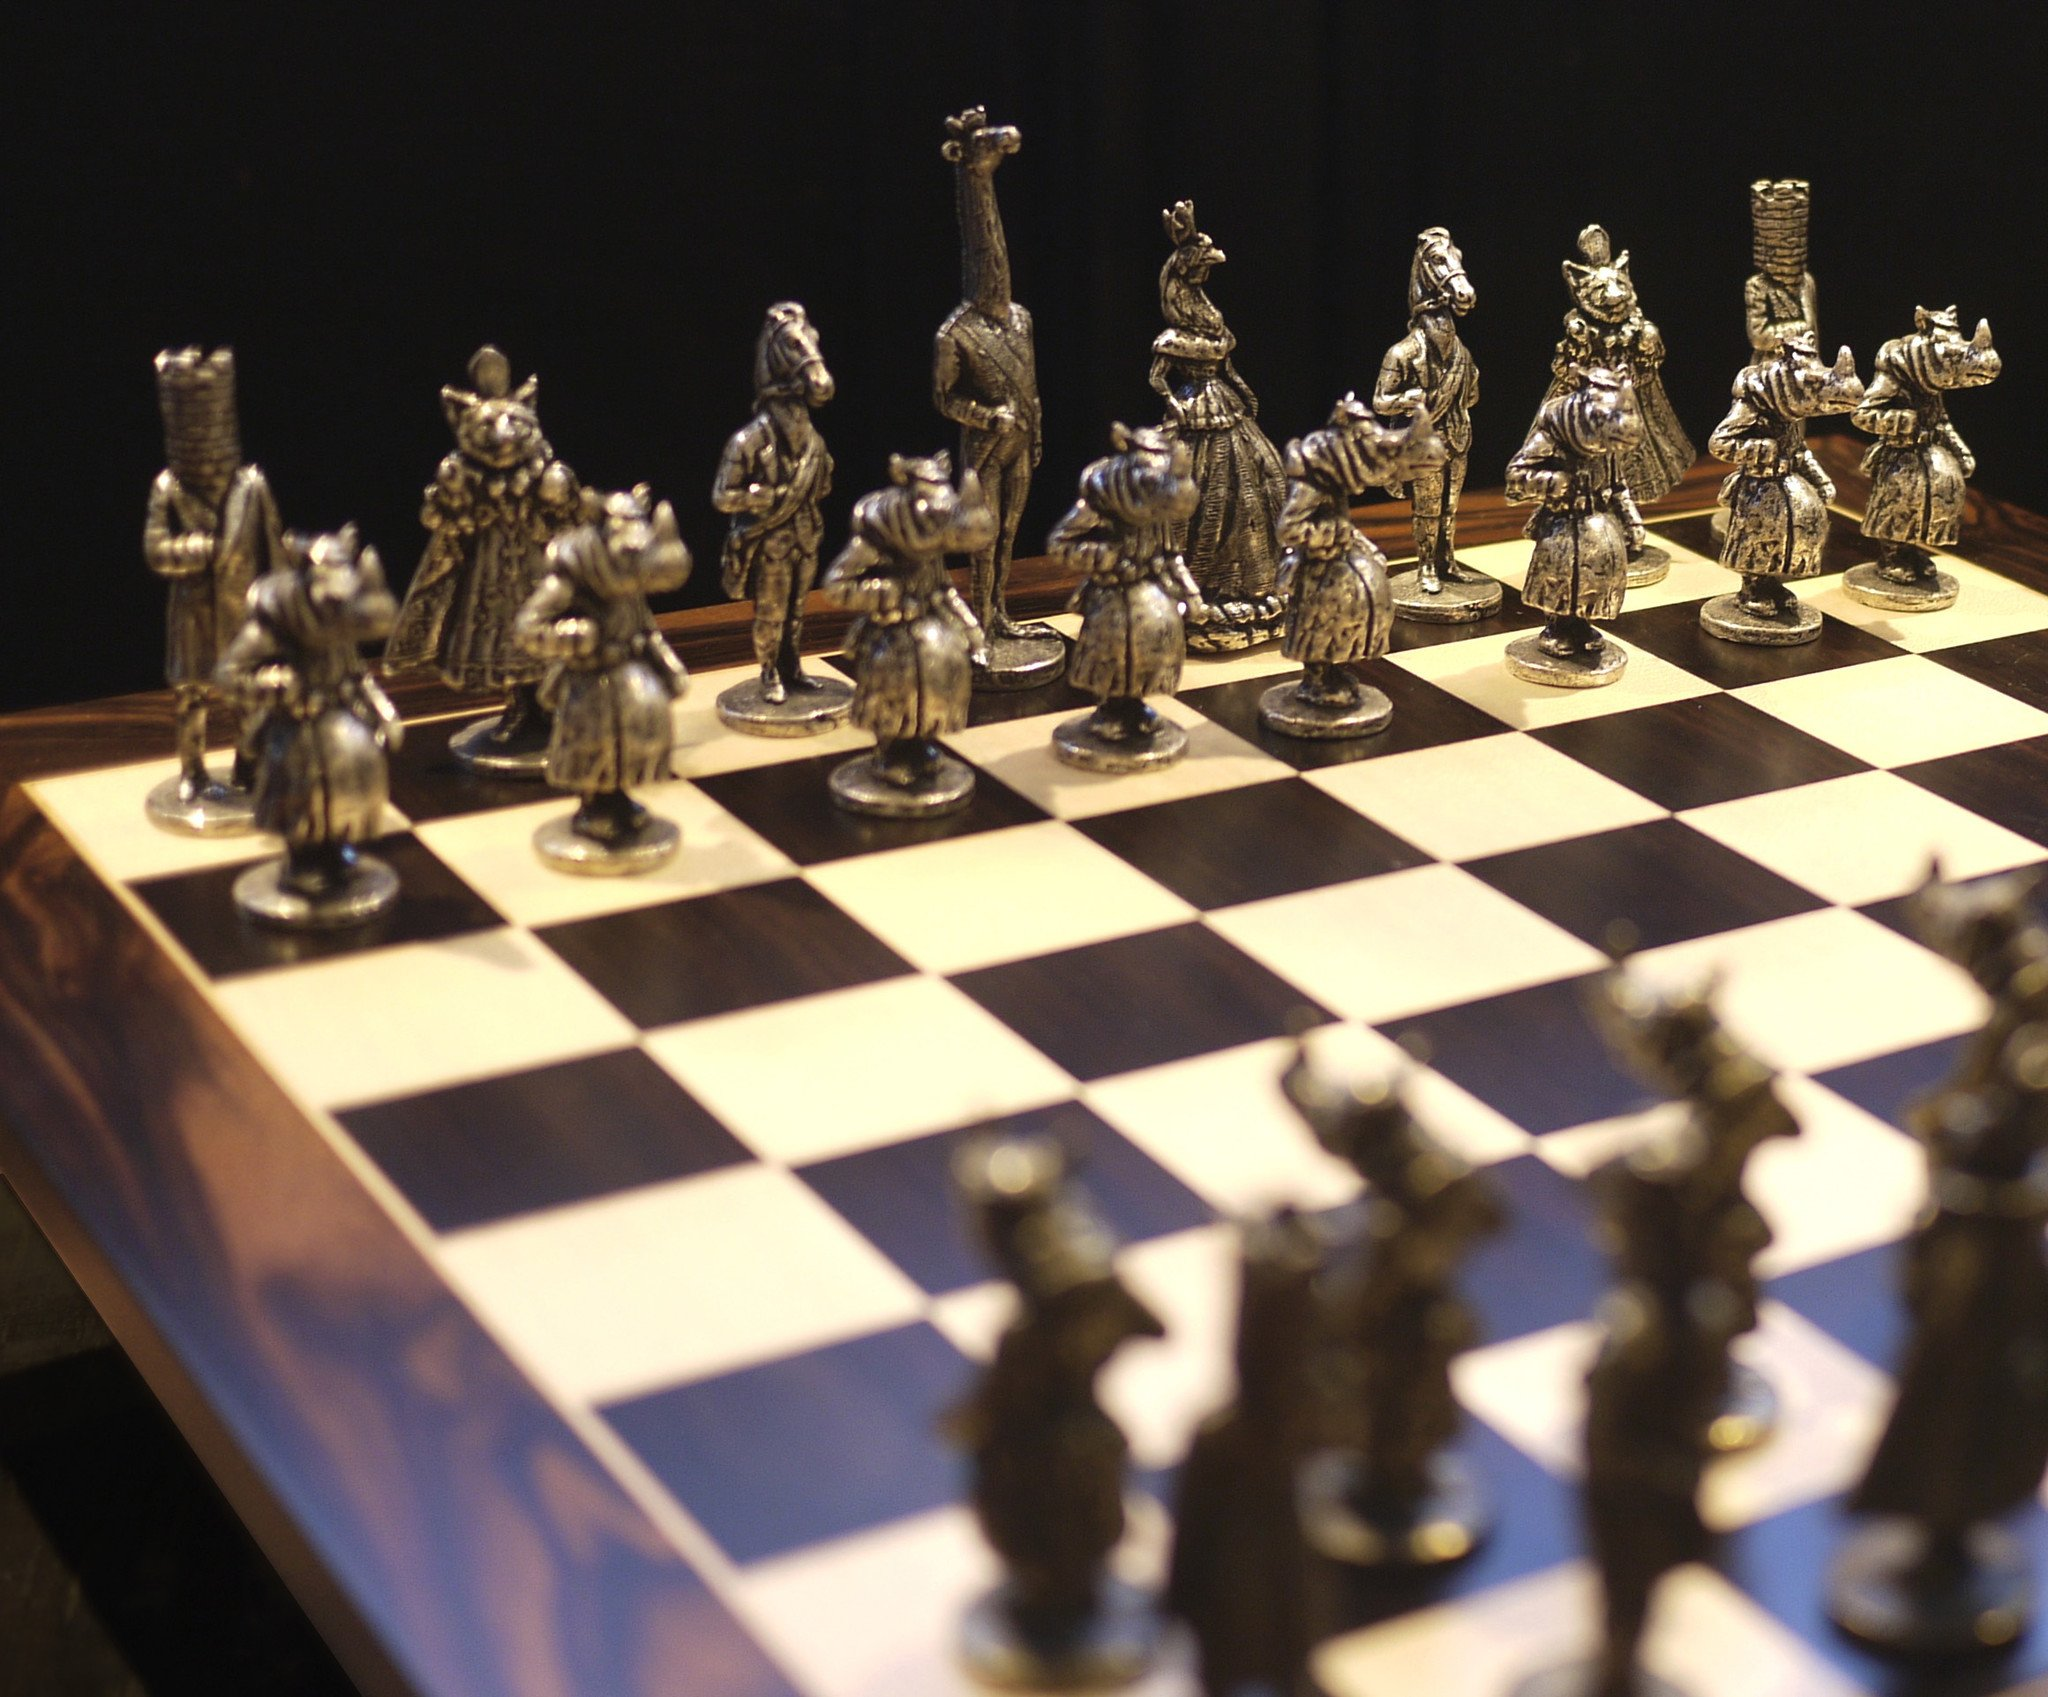
\includegraphics[scale=.1]{gfx/chess.jpg}\\\vspace{.2cm}
		\only<1>{\phantom{(if we remove draws)}}
		\only<2>{(if we remove draws)}
		\only<3>{\phantom{(if we remove draws)}}
		\only<4>{(say White wins if it's a draw)}
	\end{center}
\end{frame}

\begin{frame}{Infinite chess?}
	\begin{center}
		\only<1>{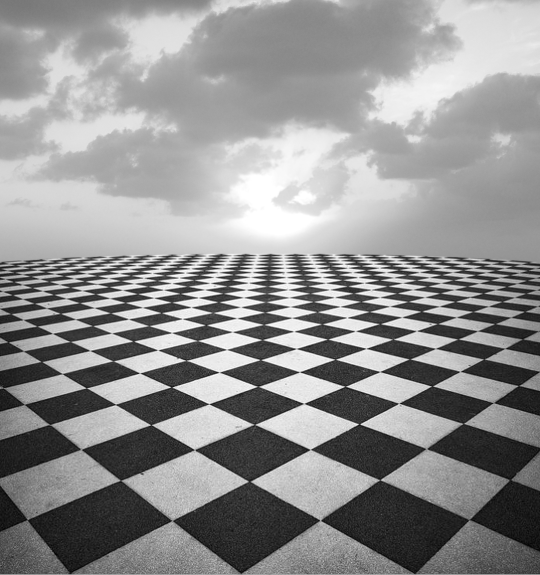
\includegraphics[scale=.37]{gfx/infinite_chess.png}}
  	\only<2->{
			\onslide<2->Same rules, same pieces, infinite board\\\vspace{.2cm}
			\onslide<3->Still determined?
		}
	\end{center}
\end{frame}

\begin{frame}{Infinite chess!}
	\begin{center}
		Note that if white loses then they've lost at a \alert<1>{finite} stage\\\vspace{.4cm}
		\pause If Black doesn't have a winning strategy then\\ White can start out by playing a \alert<2>{non-losing move}\\\vspace{.4cm}
		\pause Keep playing non-losing moves\\\vspace{.4cm}
		\pause If White loses then they've lost at a finite stage,\\ but they're playing non-losing moves, \alert<4>{contradiction!}\\\vspace{.4cm}
		\pause So \alert<5>{infinite chess is determined}
	\end{center}
\end{frame}

\begin{frame}{I know what you're thinking}
	\begin{center}
		\pause Yes, there are non-determined games out there\\\vspace{.2cm}
		\pause Let's do that another time\\\vspace{.8cm}
	\end{center}
\end{frame}

\begin{frame}
	\begin{center}
		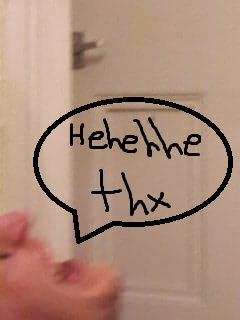
\includegraphics[scale=.8]{gfx/nick2.jpg}
	\end{center}
\end{frame}

\end{document}
